\documentclass[11pt,a4paper]{article}

\usepackage[utf8]{inputenc}
\usepackage[T1]{fontenc}
\usepackage{geometry}
\usepackage{graphicx}
\usepackage{booktabs}
\usepackage{hyperref}
\usepackage{caption}
\usepackage{float}
\usepackage{enumitem}

\geometry{margin=2.5cm}

\hypersetup{
    colorlinks=true,
    linkcolor=blue,
    urlcolor=blue,
    citecolor=blue
}

\title{\textbf{\textsc{CLARISSA}: A Conversational User Interface for Democratizing Reservoir Simulation}}

\author{
    Wolfram Laube\textsuperscript{1}, 
    Douglas Perschke\textsuperscript{2}, 
    Mike [TBD]\textsuperscript{3}\\[0.5em]
    \small\textsuperscript{1}Independent Researcher, Austria\\
    \small\textsuperscript{2}[Affiliation TBD]\\
    \small\textsuperscript{3}[Affiliation TBD]
}

\date{
    SPE Europe Energy Conference 2026\\[0.3em]
    \small Category: 05 Digital Transformation and AI\\
    \small Subcategory: 05.6 ML/AI in Subsurface Operations
}

\begin{document}

\maketitle

\begin{abstract}
Reservoir simulation remains underutilized across the full spectrum of reservoir engineering---field development planning, production surveillance, forecasting, reserves booking, and exploration risking---despite decades of software advancement. The barrier is not computational; modern solvers are fast and robust. The barrier is accessibility.

This paper introduces \textsc{CLARISSA} (Conversational Language Agent for Reservoir Integrated Simulation System Analysis), which replaces the GUI paradigm with a Conversational User Interface (CUI). Rather than requiring users to navigate software, CLARISSA enables reservoir engineers to build and iterate on simulation models through natural language dialogue---including voice input for hands-free field operations.

Recent work has demonstrated generative AI assistants that help engineers query existing models (SPE-221987). CLARISSA addresses a different problem: generating complete, validated input decks from natural language specifications. The architecture combines large language models, reinforcement learning for action optimization, and neuro-symbolic components enforcing engineering constraints.

CLARISSA executes simulations via OPM Flow, enabling license-free web-based access. To enable systematic evaluation, we introduce \textsc{RIGOR} (Reservoir Input Generation Output Review), a benchmark framework spanning coreflood models to mid-conversation compositional EOS pivots.

\textit{The binding constraint on simulation adoption has never been solver performance. It is human cognitive load and workflow friction. CLARISSA addresses that constraint directly.}
\end{abstract}

\textbf{Keywords:} Reservoir Simulation, Conversational UI, Voice Interface, Generative AI, LLM, OPM Flow, Deck Generation, Reinforcement Learning, Neuro-symbolic AI

\section{System Architecture}

The CLARISSA architecture comprises six primary layers, each addressing distinct concerns while maintaining loose coupling through well-defined interfaces (Figure~\ref{fig:architecture}).

\begin{figure}[H]
    \centering
    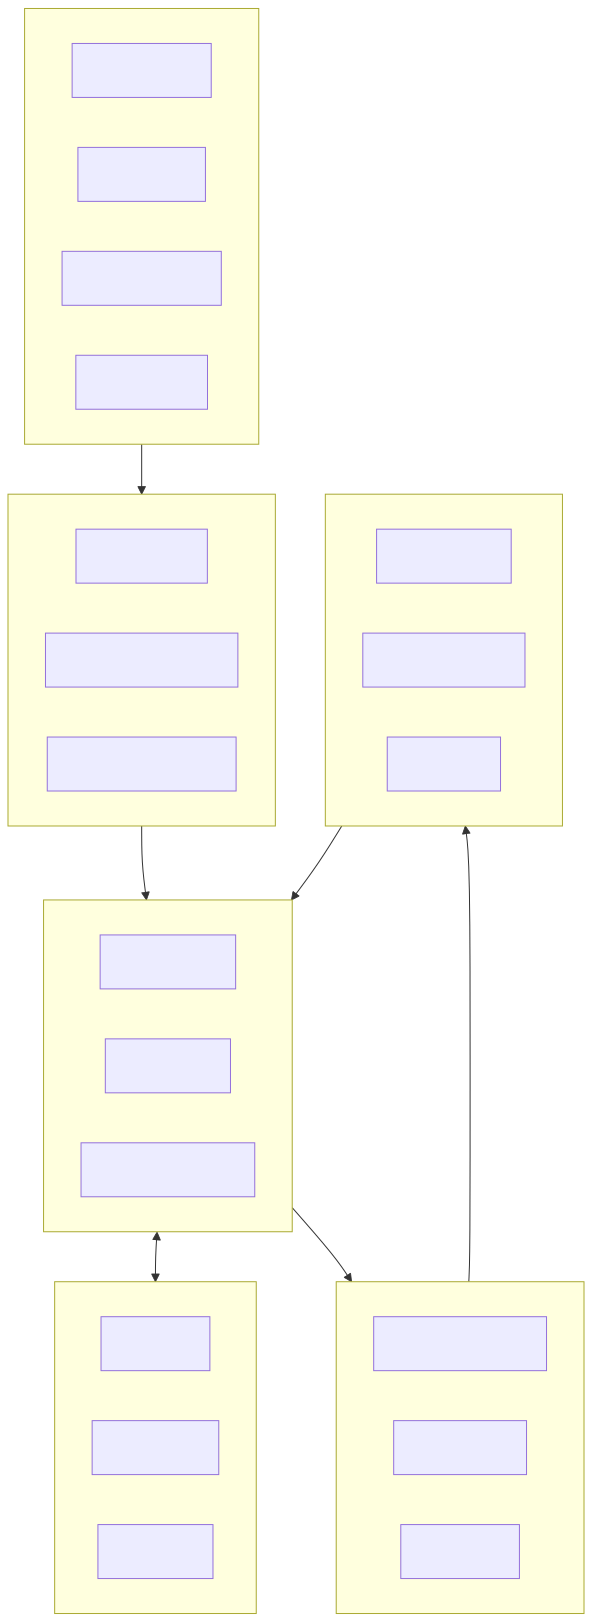
\includegraphics[width=0.95\textwidth]{diagrams/architecture-6layer.pdf}
    \caption{CLARISSA Six-Layer Architecture: User Interface (Voice, Text, Web, API), Translation, Core Processing (LLM, RL, Neuro-symbolic), Validation, Generation, and Simulation layers.}
    \label{fig:architecture}
\end{figure}

\textbf{Key Design Principles:}
\begin{itemize}[noitemsep]
    \item \textbf{Voice-First Design:} Hands-free operation from field tablets during well site visits
    \item \textbf{Graceful Degradation:} Low-confidence interpretations trigger clarification requests; failed validations roll back to last valid state
    \item \textbf{Analog-Informed Defaults:} Missing parameters suggested from basin-specific databases with explicit documentation
    \item \textbf{License-Free Execution:} OPM Flow backend enables operators without commercial licenses
\end{itemize}

\section{Development Phases}

CLARISSA evolves through three development phases (Figure~\ref{fig:phases}):

\begin{figure}[H]
    \centering
    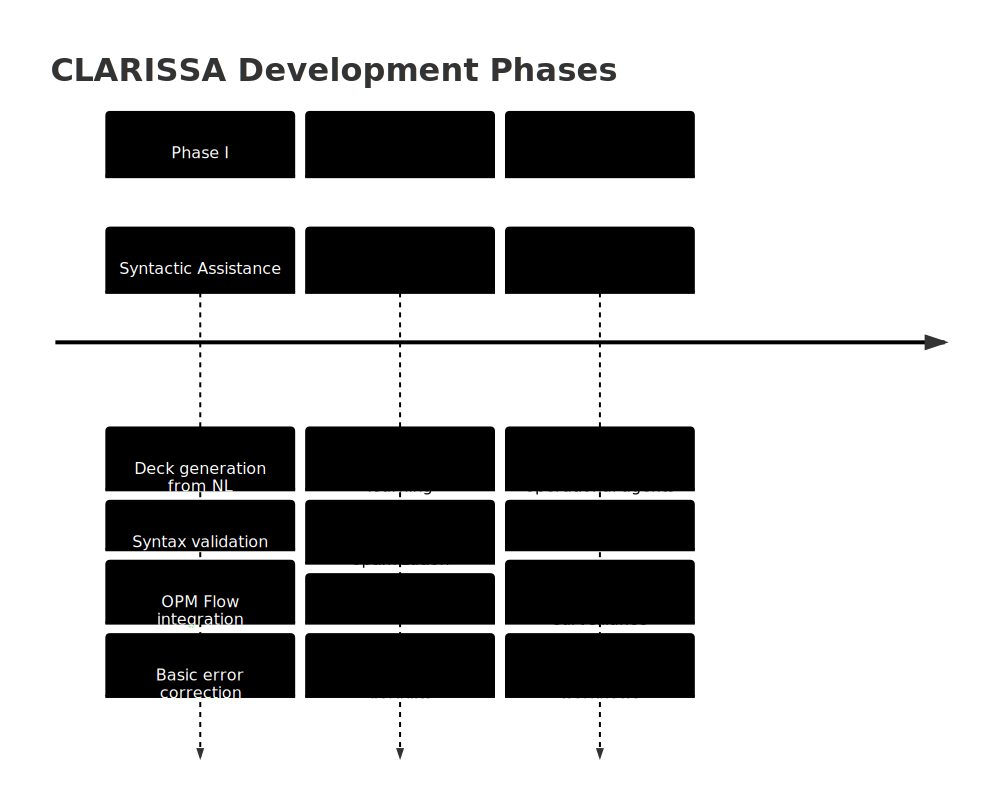
\includegraphics[width=0.85\textwidth]{diagrams/phases.pdf}
    \caption{CLARISSA Development Roadmap: Phase I (Syntactic Assistance), Phase II (Physics-Informed), Phase III (Field-Specialized).}
    \label{fig:phases}
\end{figure}

\section{Comparison with Prior Work}

Table~\ref{tab:comparison} and Figure~\ref{fig:comparison} illustrate the evolution from query-based assistants to generation-based systems.

\begin{figure}[H]
    \centering
    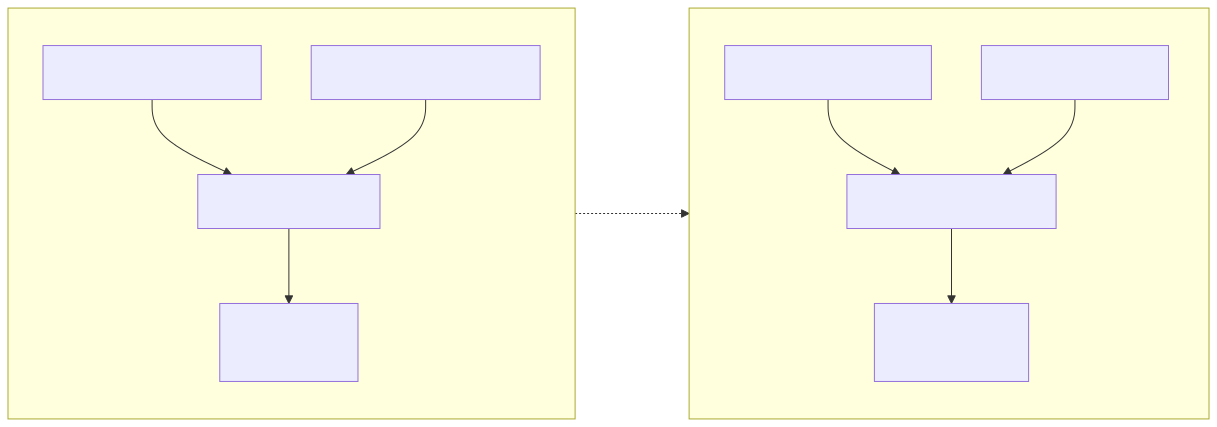
\includegraphics[width=0.8\textwidth]{diagrams/comparison.pdf}
    \caption{Evolution from Envoy (SPE-221987) to CLARISSA: Query-based vs. Generation-based paradigm.}
    \label{fig:comparison}
\end{figure}

\begin{table}[H]
\centering
\caption{Feature Comparison: Envoy vs. CLARISSA}
\label{tab:comparison}
\begin{tabular}{lll}
\toprule
\textbf{Aspect} & \textbf{Envoy (SPE-221987)} & \textbf{CLARISSA} \\
\midrule
Primary Function & Query existing models & Generate complete decks \\
Interaction Mode & Text Q\&A on loaded model & Voice + Text elicitation \\
Input Modalities & Text chat only & Voice, Text, Web, API \\
Simulator & ECHELON (proprietary) & OPM Flow (open source) \\
Architecture & RAG + Callback Agents & RL + Neuro-symbolic + Feedback \\
Learning & Static knowledge bases & Adaptive via sim feedback \\
Error Handling & Manual correction & Auto rollback + clarification \\
Validation & Post-hoc analysis & Pre-execution physics check \\
Availability & Commercial license & Web-based, license-free \\
\bottomrule
\end{tabular}
\end{table}

\section{RIGOR Benchmark Framework}

To enable systematic evaluation of CUI-based simulation systems, we introduce \textsc{RIGOR} (Reservoir Input Generation Output Review), assessing deck generation across four dimensions (Figure~\ref{fig:rigor}):

\begin{enumerate}[noitemsep]
    \item \textbf{Syntactic Validity:} Parser acceptance, keyword correctness
    \item \textbf{Semantic Correctness:} Logical consistency, unit coherence
    \item \textbf{Physical Plausibility:} Pressure gradients, saturations, rates within bounds
    \item \textbf{Conversational Efficiency:} Turns to completion, clarification rate
\end{enumerate}

\begin{figure}[H]
    \centering
    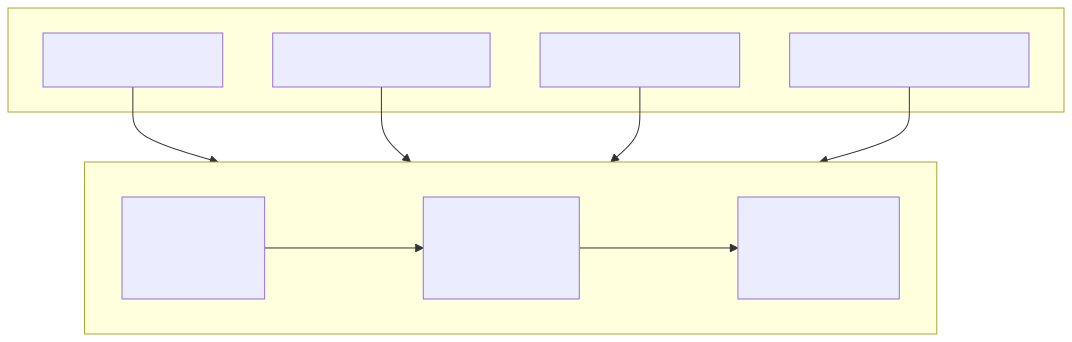
\includegraphics[width=0.75\textwidth]{diagrams/rigor.pdf}
    \caption{RIGOR Framework: Four evaluation dimensions across three complexity tiers.}
    \label{fig:rigor}
\end{figure}

\textbf{Complexity Tiers:}
\begin{description}[noitemsep]
    \item[Tier 1 (Foundational):] Linear displacement model representing laboratory coreflood
    \item[Tier 2 (Intermediate):] Pattern flood with 5-spot configuration, 40-acre spacing
    \item[Tier 3 (Advanced):] Mid-conversation conversion of black-oil waterflood to compositional EOS for tertiary recovery
\end{description}

\section{Example Interaction}

Figure~\ref{fig:conversation} demonstrates a typical voice-based field interaction sequence.

\begin{figure}[H]
    \centering
    \includegraphics[width=0.95\textwidth]{diagrams/conversation.pdf}
    \caption{Voice-based field interaction: Engineer specifies waterflood model, CLARISSA validates physics, suggests analog-based defaults, executes simulation, and offers sensitivity analysis.}
    \label{fig:conversation}
\end{figure}

\section{Conclusions}

CLARISSA represents a paradigm shift in reservoir simulation accessibility:

\begin{itemize}[noitemsep]
    \item \textbf{First CUI-based system} for complete simulation deck generation
    \item \textbf{Voice-enabled field workflows} previously impossible with traditional interfaces
    \item \textbf{License-free execution} via OPM Flow removes barriers for operators
    \item \textbf{RIGOR benchmark} provides first standardized evaluation framework
    \item \textbf{Hybrid AI architecture} combines LLM, RL, and neuro-symbolic components
\end{itemize}

\textit{The binding constraint on simulation adoption has never been solver performance. It is human cognitive load and workflow friction. CLARISSA addresses that constraint directly.}

\begin{thebibliography}{9}
\bibitem{spe221987}
K. Wiegand, M. Bedewi, K. Mukundakrishnan, D. Tishechkin, V. Ananthan, and D. Kahn,
``Using Generative AI to Build a Reservoir Simulation Assistant,''
SPE-221987-MS, ADIPEC, Abu Dhabi, 2024.

\bibitem{opm}
Open Porous Media Initiative, ``OPM Flow Documentation,'' \url{https://opm-project.org}
\end{thebibliography}

\end{document}
